\section{Introdução}
    Os robôs industriais tradicionais possuem uma arquitetura de controle fechada fornecida pelo fabricante. Esse tipo de solução segue o paradigma a qual deve ser priorizada a robustez e confiabilidade do funcionamento e da execução das tarefas, além de atender a certos requisitos normativos e legais que regem as indústrias. No entanto, é inegável que essa forma dificulta a realização de novas implementações e atividades de pesquisa com os mesmos.
    
    Algumas tentativas feitas pela academia foram relatadas na literatura no sentido de abrir a estrutura de controle de alguns robôs industriais~\citep{ROBERTI:2010}. Recentemente, alguns fabricantes de robôs perceberam essa demanda por parte das instituições de ensino e pesquisa e de forma semelhante ao que vem acontecendo com os softwares de código aberto do \textit{ROS} (Sistema Operacional Robótico, em tradução livre), oferecem a opção de abertura do sistema de controle de robôs~\citep{KUBUS:2010}, isto é, uma controladora aberta. 
    
    Uma opção para atender essa demanda foi desenvolvida pelo fabricante de robôs industriais \textit{Comau}, adicionando uma arquitetura complementar à controladora de seus robôs, a \textit{Comau C5G}. Essa extensão, denominada \textit{Comau C5G Open Controller}, é feita através da conexão da controladora a um computador industrial externo, denominado \textit{LPC (Linux Personal Computer)}, como é mostrado na Figura~\ref{controladora2}.~\citep{ANTONELLI:2010}.
    
    A Figura~\ref{controladora} permite a visualização da solução fornecida pelo fabricante, sendo que, a conexão \textit{Ethernet} TCP-IP precisa ser intermediada por um modem, roteador ou \textit{switch} não fornecido nessa extensão.
    \begin{figure}[ht]
        \centering
        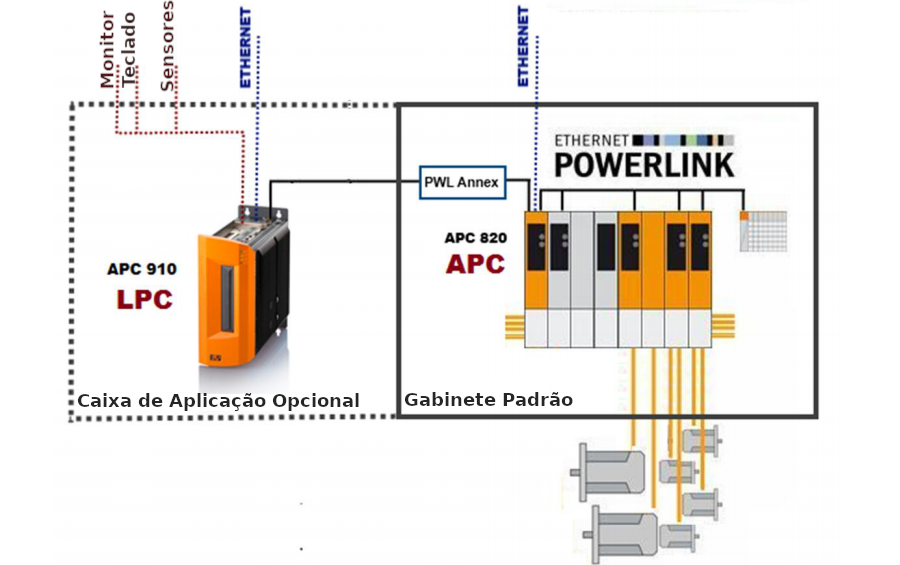
\includegraphics[width=\columnwidth]{imagens/Conexoes/controladora2.png}
        \small 
        \centering 
        \caption{Visão geral sobre o hardware do sistema C5G-Open}
        Adaptado de~\citep{Ferrara:2013}
        \label{controladora2}
    \end{figure} 
    
    Assim, é possibilitado à controladora do robô industrial enviar dados sensoriais e receber comandos de movimentação de um software a ser programado pelo usuário, a taxas de até 1 pacote a cada $0,4\,\mathrm{ms}$ (1 pacote contém todas as leituras de sensores do robô). Isso possibilita a criação de softwares que implementem malhas de controle adicionais como: controle de força, visão computacional, entre outros.~\citep{Ferrara:2013}
    
    \begin{figure}[ht]
        \centering
        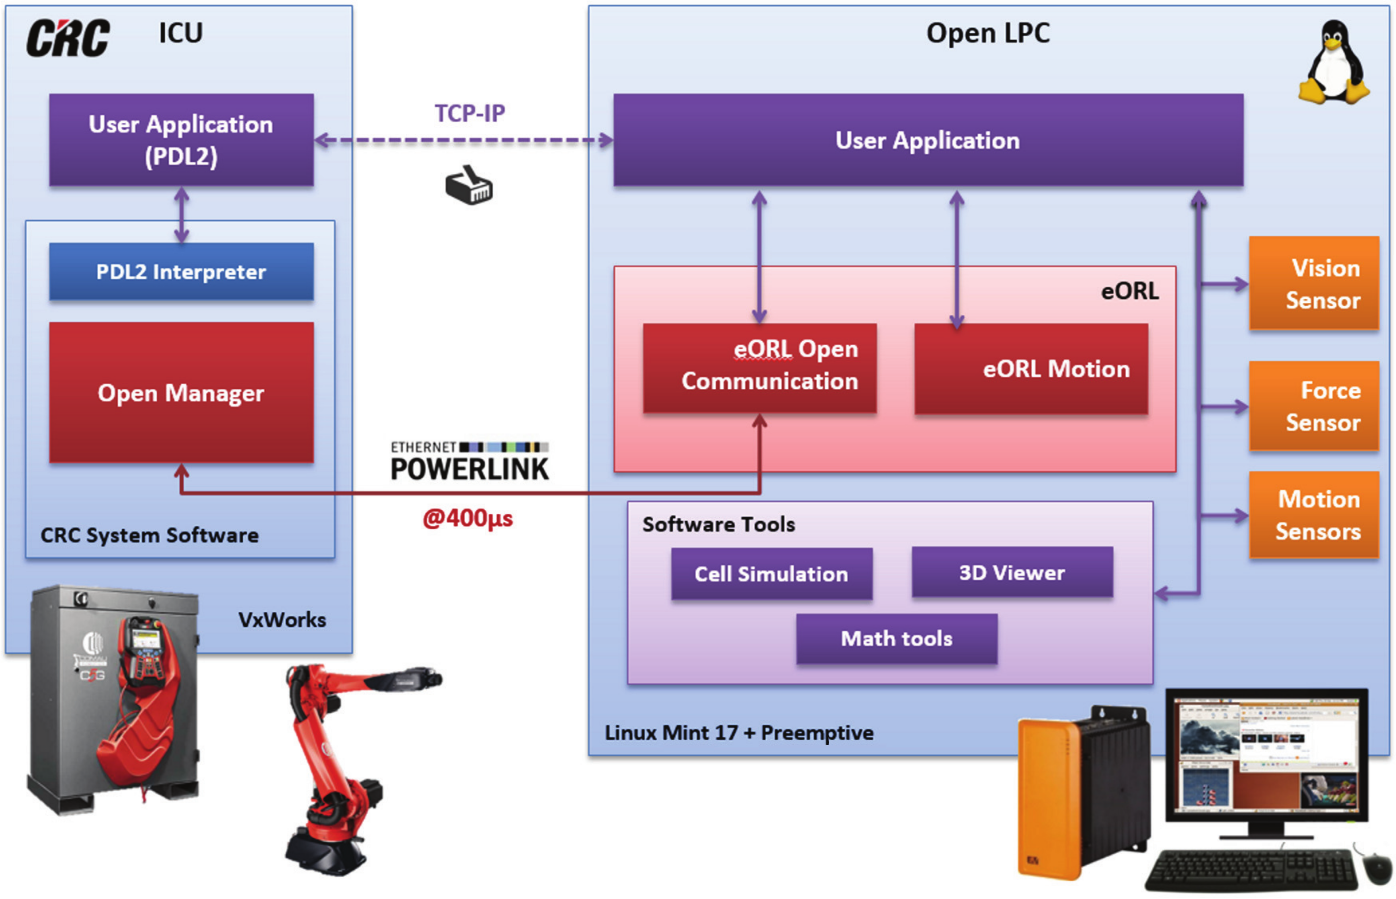
\includegraphics[width=\columnwidth]{imagens/Conexoes/controladora.png}
        \small 
        \centering 
        \caption{Visão geral do software do sistema C5G-Open}
        Fonte:~\citep{Open:Manual}
        \label{controladora}
    \end{figure} 
    
    Entretanto, existem algumas limitações, por exemplo: o software (\textit{User Application} na Figura \ref{controladora}) que implementa essa malha de controle adicional precisa ser compilado e executado nesse computador industrial externo, rodando o sistema operacional \textit{Linux Mint 17} compilado para arquitetura x86, conectado à controladora por um cabo de rede especial chamado \textit{Ethernet PowerLink} (visto na Figura \ref{controladora}). Ele precisa ser programado em C/C++ e utilizar a biblioteca proprietária de código fechado desenvolvida pela \textit{Comau} chamada \textit{eORL} (Biblioteca Robótica Realística Melhorada, em tradução livre) para controlar a comunicação.
    
    Além disso, uma utilização inadequada por um usuário que deixe a conexão com o \textit{LPC} habilitada do lado da controladora e que não tenha a adequada resposta do lado do \textit{LPC}, por exemplo, poderá produzir um erro de comunicação que acabará sendo armazenado em seus registros e impedirá a liberação dos \textit{drivers} da controladora pelo seu módulo de gerenciamento de segurança, chamado C5G-SDM (Módulo de Distribuição e Segurança, em português)~\citep{C5G:Manual}.
    
    Por fim, nem todos os programas necessários para o desenvolvimento de aplicações podem ser instalados no \textit{LPC}, como é o caso do \textit{ROS}, devido ao fato que os drivers do Powerlink Card precisam de uma versão mais antiga do Sistema Operacional Ubuntu (ou derivados dele, como Linux Mint) para funcionar~\citep{Bisson:2014}. Atualmente é executado no \textit{LPC} a versão 17 do Linux Mint, que é baseado na versão LTS (suporte de longa duração, em tradução livre) de 2014 do Ubuntu. Então, todos os programas e versões de bibliotecas do sistema operacional são versões ultrapassadas e, geralmente, não oferece suporte à instalação das novas versões dos mesmos, como é o caso do \textit{ROS 2}, que é a mais nova versão do \textit{ROS}.
    
    Visando oferecer mais liberdade e flexibilidade para o usuário, no que diz respeito à programação da malha de controle adicional e ao dispositivo que irá executá-la, foi desenvolvido um software chamado OpenServer. Este, tem também o objetivo de trazer mais segurança para a controladora do robô do laboratório do CEFET-MG em Divinópolis durante a execução de malhas de controle experimentais. Ele utiliza a biblioteca \textit{eORL} para controlar o robô e oferece uma \textit{API} (Interface de Programação de Aplicativo, em tradução livre) baseada em rede TCP/IP, o qual permite que um programa cliente em outro dispositivo controle o robô através dele. Este programa cliente pode ser escrito em qualquer linguagem de programação, compilado em qualquer arquitetura e executado em um sistema operacional de preferência. O OpenServer permite que o programa cliente leia os sensores do robô e envie os ângulos de referência para a controladora, possibilitando que o robô seja controlado até mesmo por aplicativos de \textit{smartphone} que utilizem a \textit{API}.
    
    Como mencionado acima, acredita-se que essa abordagem possa reduzir riscos ao equipamento por erro ou imperícia ao ser programada uma malha de controle usando recursos do sistema \textit{Open} fornecidos pelo fabricante. Pois, o OpenServer é programado para continuar se comunicando com a controladora, mesmo que a conexão com o programa cliente seja perdida. Além disso, ela é capaz de oferecer uma alternativa de \textit{API} mais simples de ser aprendida e utilizada.
    %na referida instituição de ensino.